%!TEX root = <main.tex>
\section{Optimizations}

In this section we explain \textit{incremental inference} and the two \textit{approximate inference} approaches, patch \textit{propagation thresholding} and \textit{adaptive drill-down}, in detail.
In \system~ these optimizations are applied on top of the current dominant approach of performing CNN inference on batches of images where each image corresponds to an occluded instance of the original image.
Batched inference is important as it reduces per image inference time by amortizing the fixed overheads.
In our experiments we found that this simple optimization alone can give up to ~1.4X speedups on CPU environments and ~2X speedups on the GPU environment compared to the per image inference approach.
Finally we explain how \system~ configures it's internal system configurations for \textit{approximate inference} by using a sample image set during the initial tuning stage.

\subsection{Incremental Inference}\label{sec:inc_computation}

As explained earlier, occlusion experiments in it's naive form performs many redundant computations.
In order to avoid these redundancies, layers in a CNN has to be change aware and operate in an incremental manner i.e. reuse previous computations as much as possible and compute only the required ones.
In this section we focus on transformations that operate on a local spatial context (i.e. Convolution and Pooling) as other types either has no redundancies (global context transformations) or is trivial to make incremental (point transformations).
The choice of CPUs vs GPUs for CNN inference also brings up new considerations for the batched implementation of these incremental transformations and we explain two version of implementations, one which is a naive implementation of batched incremental inference approach and the other a GPU optimized version.
We also explain incremental implementations of two other linear algebra operators, input volume addition and depth-wise concatenation, which are also two popular operators seen in CNN architectures.

\vspace{2mm}
\noindent \textbf{Incremental Convolution and Pooling.}


\begin{table}[t]
  \centering
  \caption{Additional symbols used in the Optimizer Section}
  \scalebox{0.8}{\begin{tabular}{p{2cm}p{7.5cm}}
    \toprule
    \textbf{Symbol} & \textbf{Meaning}\\
    \midrule \midrule
    $x^I_P,y^I_P$ & Starting coordinates of the input patch\\
    \midrule
    $x^R_P,y^R_P$ & Starting coordinates of the patch that needs to be read in for the transformation\\
    \midrule
    $x^O_P,y^O_P$ & Starting coordinates of the output patch\\
    \midrule
    $H^I_P,W^I_P$ & Height, and width of the input patch\\
   	\midrule
   	$H^R_P,W^R_P$ & Height, and width of the patch that needs to be read in for the transformation\\
   	\midrule
   	$H^O_P,W^O_P$ & Height, and width of the output patch\\
    \bottomrule
  \end{tabular}}
\label{table:optimizer_symbols}
\end{table}


\begin{figure}[t]
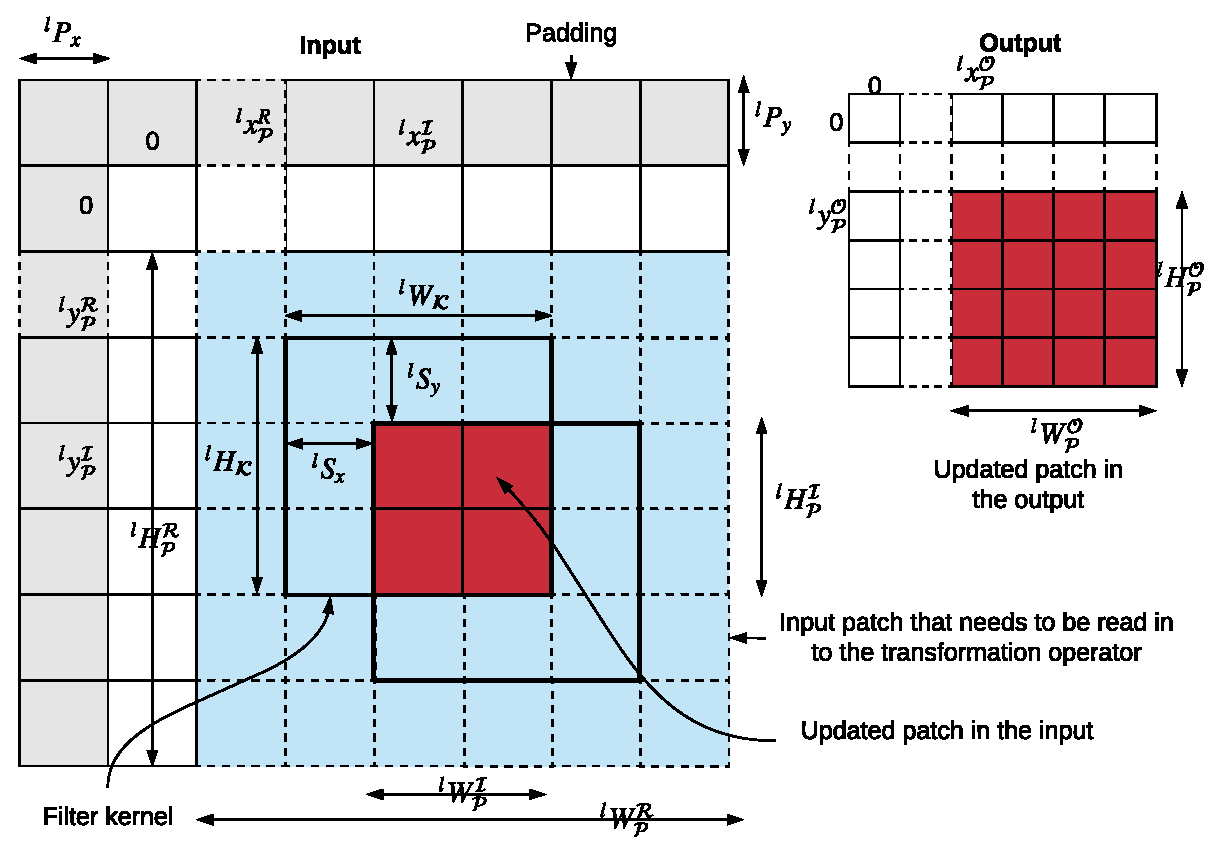
\includegraphics[width=\columnwidth]{images/dimensions}
\caption{Simplified representation of input and output patch coordinates and dimensions of Conv. and Pool transformations.}
\label{fig:dimensions}
\end{figure}

The two types of transformations in a CNN that operate on a local spatial context are Convolution and Polling. In Section \ref{sec:preliminaries} we showed that both of these transformations can be cast into a form of applying a filter along the spatial dimensions of the input volume.
However how each transformation operate along the depth dimension is different.
For our purpose we are interested in finding the propagation of the patches in the input through the consecutive layers and hence both these transformations can be treated similarly.
The coordinates and the dimensions (i.e. height and width) of the modified patch in the output volume caused by a modified patch in the input volume are determined by the coordinates and the dimensions of the input patch, sizes of the filter kernel ($H_k$ and $W_k$), padding values ($P_x$ and $P_y$), and the strides ($S_x$ and $S_y$).
For example consider simplified demonstration showing a cross-section of input and output in Figure \ref{fig:dimensions}.
We use a coordinate system whose origin is placed at the top left corner of the input.
A patch is placed on the input starting off at $x^I_P, y^I_P$ coordinates and has a height of $H^I_P$ and width of $W^I_P$.
The updated patch in the output starts off at $x^O_P, y^O_P$ and has a height of $H^O_P$ and width of $W^O_P$.
Note that due to the overlapping nature of filter positions, to compute the output patch, transformations may have to read a slightly larger context than the input patch. This read in context is shown by the blue shaded area in Figure \ref{fig:dimensions}.
The starting coordinates of this read-in patch are denoted by $x^R_P, y^R_P$ and the dimensions are denoted by $W^R_P, H^R_P$.
The relationship between the coordinates and dimensions can be expressed as follows:

\begin{align}
\label{eqn:xcoordinate}
x^O_P =&~ max\big(\lceil (P_x + x^I_P - W_K + 1)/S_x \rceil, 0\big)\\
\label{eqn:ycoordinate}
y^O_P =&~ max\big(\lceil (P_y + y^I_P - H_K + 1)/S_y \rceil, 0\big)\\
\label{eqn:patchwidth}
W^O_P =&~ min\big(\lceil (W^I_P + W_K - 1)/S_x \rceil, W_{out}\big)\\
\label{eqn:patchheight}
H^O_P =&~ min\big(\lceil (H^I_P + H_K - 1)/S_y \rceil, H_{out}\big)\\
\label{eqn:xreadcoordinate}
x^R_P =&~ x^O_P \times S_x - P_x\\
\label{eqn:yreadcoordinate}
y^R_P =&~ y^O_P \times S_y - P_y\\
\label{eqn:readpatchwidth}
W^R_P =&~ W_K + (W^O_P-1) \times S_x\\
\label{eqn:readpatchheight}
H^R_P =&~ H_K + (H^O_P-1) \times S_y
\end{align}


Equation \ref{eqn:xcoordinate} and \ref{eqn:ycoordinate} calculates the starting coordinates of the output patch.
Use of padding effectively shifts the coordinate system and therefore $P_x$ and $P_y$ values are added to correct it.
Due to the overlapping nature of filter kernels, the maximum affected span of the updated patch in the input will be increased by $W_K-1$ and $H_K-1$ amounts and hence needs to be subtracted from the input coordinates $x^I_P$ and $y^I_P$ (a filter of size $W_K$ which is placed starting at $x^I_P - W_K + 1$ will see the new change at $x^I_P$).
Dividing the above values by the stride values $S_x$ and $S_y$ and taking the \texttt{ceil} gives the starting coordinates of the output patch (essentially calculates the number of strides).
Towards the left side edge of the input, where the affected span of the input cannot be extended by $W_k-1$ or $H_K-1$ amounts this value will be negative.
Therefore the maximum of zero or the above value should be taken as the final.
Equation \ref{eqn:patchwidth} and \ref{eqn:patchheight} calculates the width and height of the output patches.
Similar to output coordinates calculations, the span of the input patch is increased by $W_K-1$ and $H_K-1$ amounts.
Dividing the above values by the stride values $S_x$ and $S_y$ and taking the \texttt{ceil} gives the width and height of the output patch.
Since the output patch cannot grow beyond the size of the output, minimum of the output dimension or the above value should be taken as the final.
Once the output patch coordinates and dimensions are calculated, it is straight forward to calculate the read-in patch coordinates as per Equations \ref{eqn:xreadcoordinate} and \ref{eqn:yreadcoordinate} and the dimensions as per Equations \ref{eqn:readpatchwidth} and \ref{eqn:readpatchheight}.


\begin{figure}[t]
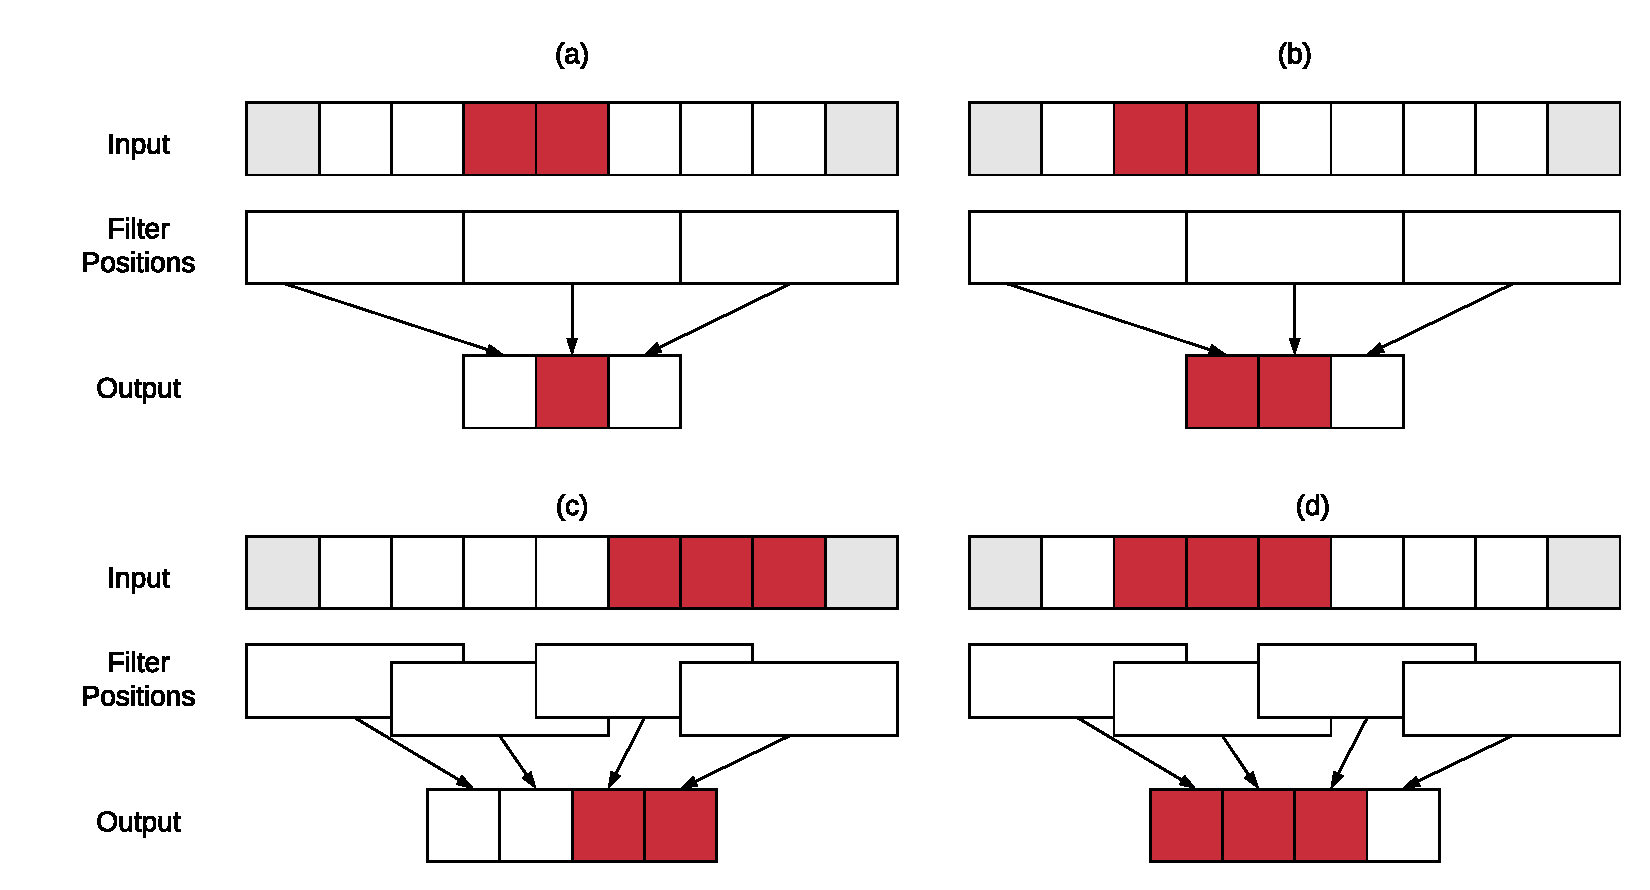
\includegraphics[width=\columnwidth]{images/less_one_example}
\caption{One dimensional representation showing special situations under which actual output size will be smaller than the values calculated by Equations \ref{eqn:xcoordinate} and \ref{eqn:ycoordinate}. (a) and (b) shows a situation with filter stride being equal to the filter size. (c) and (d) shows a situation with input patch being placed at the edge of the input.}
\label{fig:less_one_example}
\end{figure}

It is important to note that there are special situations under which the actual output patch size can be smaller than above calculated value. Consider the simplified one dimensional situation shown in Figure \ref{fig:less_one_example} (a), where the stride value\footnote{Note that the stride value is generally less than or equal to the filter size.} (3) is same as the filter size (3). In this situation the the size of the output patch is one less than the value calculated by Equation \ref{eqn:patchwidth}. However it is not the case in Figure \ref{fig:less_one_example} (b) which has the same input patch size but is placed at a different location. This issue arises only when the stride value is same as the filter size.
Another situation arises when the input patch is placed at the edge of the input as shown in Figure \ref{fig:less_one_example} (c). In this situation it is not possible for the filter to move freely through all filter positions as it hits the input boundary compared to having the input patch on the middle of the input as shown in Figure \ref{fig:less_one_example} (c).
In \system~ we do not distinguish theses differences and use the values calculated by Equation \ref{eqn:patchwidth} and \ref{eqn:patchheight} as they act as an upper bound. In case of a smaller output patch, \system~ simply reads off and updates slightly bigger patches to preserve uniformity.
This also requires updating the starting coordinates of the patches as shown in Equations \ref{eqn:width_subtract} and \ref{eqn:height_subtract}.
Such uniform treatment is required for performing batched inference operations which out of the box gives significant speedups compared to per image inference.

\vspace{2mm}
\hspace{4mm} If $x^O_P + W^O_P > W_{out}:$
\begin{align}
\label{eqn:width_subtract}
x^O_P = &~ W_{out} - W^O_P\\
x^I_P = &~ W_{in} - W^I_P\\
x^R_P = &~ W_{in} - W^R_P
\end{align}

\hspace{4mm} If $y^O_P + H^O_P > H_{out}:$
\begin{align}
\label{eqn:height_subtract}
y^O_P = &~ H_{out} - H^O_P\\
y^I_P = &~ H_{in} - H^I_P\\
y^R_P = &~ H_{in} - H^R_P
\end{align}


\begin{algorithm}
    \caption{Incremental Inference Algorithm}\label{euclid}
    \begin{flushleft}
     \hspace*{4mm} \textbf{Input:} \\
     \hspace*{8mm} $T$ : \textit{Transformation}\\
     \hspace*{8mm} $I$ : \textit{Pre-materialized input from original image}\\
     \hspace*{8mm} $[P^I_1,...,P^I_n]$ : \textit{Input patches}\\
     \hspace*{8mm} $[(x^I_{P_1},y^I_{P_1}),...,(x^I_{P_n},y^I_{P_n})]$ : \textit{Input patch coordinates}\\
     \hspace*{8mm} $W^I_P,H^I_P$ : \textit{Input patch dimensions}
    \end{flushleft}

	\begin{flushleft}
     \hspace*{4mm} \textbf{Output:}\\
     \hspace*{8mm} $[P^O_1,...,P^O_n]$ : \textit{Output patches}\\
     \hspace*{8mm} $[(x^O_{P_1},y^O_{P_1}),...,(x^O_{P_n},y^O_{P_n})]$ : \textit{Output patch coordinates}\\
     \hspace*{8mm} $W^O_P,H^O_P$ : \textit{Output patch dimensions}
    \end{flushleft}

    \begin{algorithmic}[1]
    \Procedure{IncrementalInference}{}
    \State \textit{Calculate} $[(x^O_{P_1},y^O_{P_1}),...,(x^O_{P_n},y^O_{P_n})]$ \textit{and} ($W^O_P,H^O_P$)
    \State \textit{Calculate} $[(x^R_{P_1},y^R_{P_1}),...,(x^R_{P_n},y^R_{P_n})]$ \textit{and} ($W^R_P,H^R_P$)
    \State \textit{Initialize} $R \in \mathcal{\rm I\!R}^{\texttt{depth}(I) \times H^R_P \times W^R_P}$

    \For{\texttt{i in [1,...,n]}}
    	\State $t_1 \gets I[:,x^R_{P_i}:x^R_{P_i}+W^R_P,y^R_{P_i}:y^R_{P_i}+H^R_P]$ 
    	\State $t_2 \gets P_i \bm\circ_{(x^I_{P_i}-x^R_{P_i}),(y^I_{P_i}-y^R_{P_i})} t_1$
    	\State $R[i,:,:] \gets t_2$
    \EndFor

    \State $[P^O_1,...,P^O_n] \gets T(R)$
    \State \textbf{return} $[P^O_1,...,P^O_n]$, $[(x^O_{P_1},y^O_{P_1}),...,(x^O_{P_n},y^O_{P_n})],$
    \State \hspace*{20mm} ($W^O_P,H^O_P$) 
    \EndProcedure
    \end{algorithmic}

    \vspace*{-2mm}
    \hrulefill
    
    \begin{flushleft}
     \hspace*{4mm} \textbf{Input:}\\
     \hspace*{8mm} $O$ : \textit{Pre-materialized output from original image}\\
     \hspace*{8mm} $[P^O_1,...,P^O_n]$ : \textit{Output patches}\\
     \hspace*{8mm} $[(x^O_{P_1},y^O_{P_1}),...,(x^O_{P_n},y^O_{P_n})]$ : \textit{Output patch coordinates}\\
    \end{flushleft}

    \begin{flushleft}
     \hspace*{4mm} \textbf{Output:}\\
     \hspace*{8mm} $O\textrm'$ : \textit{Updated output}
    \end{flushleft}
	\begin{algorithmic}[1]
    \Procedure{IncrementalToFullProjection}{}
    \State $O\textrm' \gets \texttt{copy}(O)$
    \For{\texttt{i in [1,...,n]}}
    	\State $O\textrm'[i,:,:] \gets P^O_i \bm\circ_{x^O_{P_i},y^O_{P_i}} O\textrm'[i,:,:]$
    \EndFor
    \State \textbf{return} $O\textrm'$
    \EndProcedure

    \end{algorithmic}
\end{algorithm}

\subsection{Projective Field Thresholding}

\subsection{Adaptive Drill-Down}

\subsection{System Tuning}
